\documentclass[tikz,border=3pt]{standalone}
\usepackage{lmodern}
\usepackage{xcolor}
\usetikzlibrary{arrows.meta}

\definecolor{cRed}{HTML}{FADBD8}
\definecolor{cYellow}{HTML}{FEF9E7}
\definecolor{cGreen}{HTML}{D5F5E3}

\begin{document}
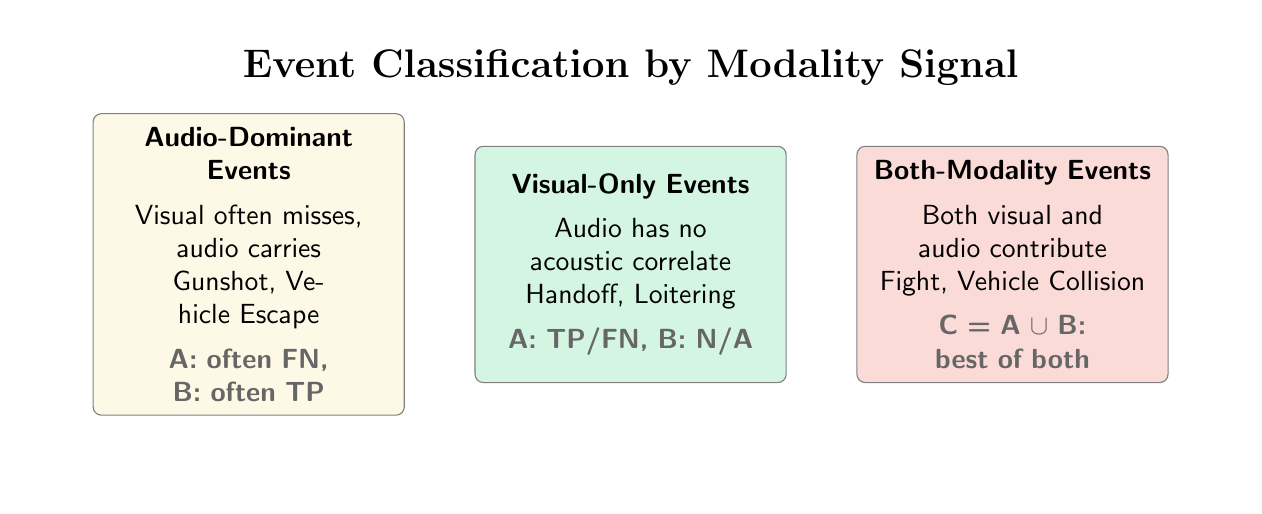
\begin{tikzpicture}[
  every node/.style={font=\sffamily},
  box/.style={draw=black!50, rounded corners=3pt, align=center, inner sep=5pt, text width=3.6cm, minimum height=3cm},
]

\draw[white] (-0.3,-0.3) rectangle (15.0,5.5);
\node[font=\Large\bfseries] at (7.35,5.0) {Event Classification by Modality Signal};

\node[box,fill=cYellow] at (2.5,2.5) {
    \textbf{Audio-Dominant Events}\\[4pt]
    Visual often misses, audio carries\\Gunshot, Vehicle Escape\\[4pt]
    \textbf{\textcolor{black!60}{A: often FN, B: often TP}}
};
\node[box,fill=cGreen] at (7.35,2.5) {
    \textbf{Visual-Only Events}\\[4pt]
    Audio has no acoustic correlate\\Handoff, Loitering\\[4pt]
    \textbf{\textcolor{black!60}{A: TP/FN, B: N/A}}
};
\node[box,fill=cRed] at (12.2,2.5) {
    \textbf{Both-Modality Events}\\[4pt]
    Both visual and audio contribute\\Fight, Vehicle Collision\\[4pt]
    \textbf{\textcolor{black!60}{C = A $\cup$ B: best of both}}
};

\end{tikzpicture}
\end{document}
